%
%  Erik Olsen
% Chris Thoma
\documentclass[12pt,fullpage]{article}
\usepackage{fullpage}                                        % use all of the page for text 
\usepackage{psfrag}                                          % LaTeX graphics tool
\usepackage{pslatex}                                         % avoids the default cmr font
\usepackage{graphicx}                                        % graphics package 
\usepackage{epsfig}                                          % figures
\usepackage{hyperref}
\usepackage{color}

\begin{document}

\noindent
{\bf Hypoexponential distribution} (from \color{blue}\url{http://www.math.wm.edu/~leemis/chart/UDR/UDR.html}\color{black})

\noindent
The shorthand $X \sim$ hypoexponential$(\vec{\alpha})$ is used to indicate that the
random variable $X$ has the hypoexponential distribution with positive vector
parameter $\vec \alpha$ such that $\alpha_{\kern 0.08 em i}\neq \alpha_j\  {\rm for}\  i \neq j$.  
If $T_i\sim$~exponential($\alpha_i$) for~$i=1,2,\ldots,n$, and $T_1, \, T_2, \, \ldots , \, T_n$ are
mutually independent random variables, then $T=T_1+T_2+\cdots+T_n$ has the hypoexponential distribution.
A hypoexponential random variable $X$ has probability density function 
$$
f(x) = \sum_{i\,=\,1}^n(1/\alpha_{\kern 0.08 em i})e^{-x/\alpha_{\kern 0.08 em i}}\left(\prod_{j\,=\,1,\,j \, \neq \,  i}^n \frac{\alpha_{\kern 0.08 em i}}{\alpha_{\kern 0.08 em i}-\alpha_j}\right)
$$
for $x>0$. The probability density function for $\vec \alpha = (0.25, \, 0.5, \, 1)$ is illustrated below.

\begin{figure}[h!]
\begin{center}
\psfrag{labf}{$f(x)$}
\psfrag{labx}{$x$}
\includegraphics[width=3.2in]{HypoexponentialPlot.ps}
\end{center}
\end{figure}

\noindent
For the case where $n=2$, the cumulative distribution function on the support of $X$ is
$$
F(x) = P(X \leq x) = 1 - \frac{1}{\alpha_1 - \alpha_2} \left( \alpha_2 e^{-x/\alpha_2} - \alpha_1 e^{-x/\alpha_1} \right)
\qquad \qquad x > 0.
$$
The general cumulative distribution, survivor, hazard, cumulative hazard, moment generating, and characteristic functions on the support of $X$ are mathematically intractable.
\vspace{0.1in}

\noindent
The population mean, variance, and skewness of $X$ are
$$
E[X] = \displaystyle \sum_{i\,=\,1}^n \alpha_{\kern 0.08 em i} \qquad \qquad 
V[X] =  \displaystyle \sum_{i\,=\,1}^n \alpha_{\kern 0.08 emi}^{\kern 0.08 em 2}  \qquad \qquad 
E\left[ \left( \frac{X - \mu}{\sigma} \right) ^ 3 \right] = \frac{2 \displaystyle \sum_{i\,=\,1}^n \alpha_{\kern 0.08 em i}^{\kern 0.08 em 3}}{\left( \displaystyle \sum_{i\,=\,1}^n \alpha_{\kern 0.08 em i}^{\kern 0.08 em 2}\right)^{\kern -0.08 em 3/2}}. \quad \quad
$$
\vspace{0.1in}

\newpage
\noindent
{\bf APPL verification:}
The APPL statements
\begin{verbatim}
X:= HypoExponentialRV([1 / alpha1, 1 / alpha2, 1 / alpha3]);
Mean(X);
Variance(X);
Skewness(X);
\end{verbatim}
verify the population mean, variance, and skewness for the special case of $n=3$.
\end{document}
